\documentclass[11pt,a4paper]{article}
\usepackage[utf8]{inputenc}
\usepackage[T1]{fontenc}
\usepackage{mathptmx}
\usepackage{amsmath,amssymb}
\usepackage{graphicx}
\usepackage{booktabs}
\usepackage{hyperref}
\usepackage[margin=1in]{geometry}
\usepackage{natbib}
\usepackage{algorithm}
\usepackage{algorithmic}
\usepackage{xcolor}
\usepackage{caption}
\usepackage{subcaption}

\title{ImmunoSim: Gymnasium Environments for Reinforcement Learning\\in Cancer Immunotherapy Optimization}
\author{Hass Dhia\\
Smart Technology Investments Research Institute\\
\texttt{partners@smarttechinvest.com}}
\date{March 2026}

\begin{document}
\maketitle

% ============================================================
% 1. ABSTRACT
% ============================================================
\begin{abstract}
Cancer immunotherapy treatment scheduling presents a sequential decision-making problem where clinicians must balance tumor control against immune-related adverse events across multiple treatment cycles.
Despite the natural fit between reinforcement learning (RL) and treatment optimization, no publicly available Gymnasium-compatible environment suite exists for immunotherapy-specific scheduling.
We present \textsc{ImmunoSim}, an open-source Python package providing four Gymnasium environments spanning anti-PD-1 monotherapy, dual checkpoint blockade (PD-1 + CTLA-4), CAR-T cell infusion optimization, and adaptive dosing with pseudo-progression handling, each grounded in validated ODE models from the tumor immunology literature.
PPO agents trained on ImmunoSim achieve 1.14--1.59$\times$ improvement over random baselines across all environments, with the dual checkpoint blockade environment showing the strongest learning signal (1.59$\times$) due to asymmetric toxicity profiles that create steeper reward gradients.
The package, including 175 passing tests, training pipelines, and clinical heuristic baselines, is available at \url{https://github.com/HassDhia/immunosim} under the MIT license.
\end{abstract}

% ============================================================
% 2. INTRODUCTION
% ============================================================
\section{Introduction}

Immune checkpoint inhibitors (ICIs) have transformed cancer treatment over the past decade, with anti-PD-1 (nivolumab, pembrolizumab) and anti-CTLA-4 (ipilimumab) agents producing durable responses in melanoma, non-small cell lung cancer, and dozens of other malignancies. CAR-T cell therapy has achieved remarkable complete remission rates in hematological cancers. However, both modalities present challenging scheduling decisions: when to dose, how much to dose, when to combine, and when to pause treatment.

Current clinical protocols rely on fixed schedules (e.g., nivolumab 3 mg/kg every 2 weeks) derived from dose-finding trials that optimize for population-level safety, not individual-patient efficacy. Reinforcement learning offers a principled framework for discovering adaptive, patient-responsive dosing strategies that could outperform fixed protocols.

The RL-immunotherapy intersection remains underexplored. While RL has been applied to chemotherapy scheduling \citep{Eastman2021, Engelhart2011}, immunotherapy-specific RL environments do not exist as standardized, publicly available Gymnasium packages. This gap limits reproducibility, benchmarking, and progress.

We present \textsc{ImmunoSim}, a Python package providing four Gymnasium-compatible RL environments for cancer immunotherapy optimization:

\begin{enumerate}
    \item \textbf{CheckpointInhibitor-v0}: Anti-PD-1 monotherapy dosing using Kuznetsov-Taylor-Perelson tumor-immune dynamics \citep{Kuznetsov1994} with Nikolopoulou PD-1 pharmacodynamics \citep{Nikolopoulou2018}.
    \item \textbf{CombinationTherapy-v0}: Dual anti-PD-1 + anti-CTLA-4 blockade with synergy modeling \citep{Nikolopoulou2021} and asymmetric toxicity profiles \citep{Shulgin2020}.
    \item \textbf{CARTCell-v0}: CAR-T cell infusion optimization using the CARTmath model \citep{Barros2021} with cytokine release syndrome toxicity \citep{Santurio2025}.
    \item \textbf{AdaptiveDosing-v0}: Adaptive response-based dosing with pseudo-progression handling via the Butner-Cristini patient model \citep{Butner2020}.
\end{enumerate}

% ============================================================
% 3. RELATED WORK
% ============================================================
\section{Related Work}

\subsection{Tumor-Immune ODE Models}

The mathematical modeling of tumor-immune interactions traces to Stepanova (1980) and was formalized by Kuznetsov, Taylor, Makalkin, and Perelson \citeyearpar{Kuznetsov1994}, who developed a two-ODE system with Michaelis-Menten immune stimulation and bilinear kill terms, fitted to BCL1 lymphoma data. \citet{dePillis2001} extended this to a four-population system with optimal control, and \citet{dePillis2005} validated an expanded model against human data distinguishing NK cells from CD8+ T cells.

\subsection{Checkpoint Inhibitor Pharmacodynamics}

\citet{Nikolopoulou2018} produced the first dedicated ODE model of PD-1/PD-L1 checkpoint inhibitor dynamics, demonstrating that anti-PD-1 monotherapy is often insufficient for tumor eradication. \citet{Nikolopoulou2021} extended this to combination ICI + immunostimulant therapy, showing sub-additive dosing requirements. \citet{Milberg2019} developed a comprehensive QSP model integrating CTLA-4, PD-1, and PD-L1 blockade. \citet{Shulgin2020} quantified a key clinical asymmetry: CTLA-4 inhibitors exhibit dose-dependent toxicity while PD-1 inhibitors do not.

\subsection{CAR-T Cell Modeling}

\citet{Barros2021} developed CARTmath, a four-compartment ODE model capturing CAR-T cell injection, activation, memory differentiation, and tumor kill. \citet{Santurio2025} extended this to include macrophage-mediated cytokine release syndrome, identifying the CAR-T/macrophage interaction as the key CRS driver.

\subsection{RL for Cancer Treatment Optimization}

\citet{Eastman2021} demonstrated that RL-derived dosing schedules are more robust to patient parameter uncertainty than classical optimal control solutions. \citet{Engelhart2011} established optimal control baselines for cancer chemotherapy ODEs. \citet{Butner2020} showed that mechanistic models can predict clinical outcomes with 88\% accuracy from standard imaging, validating the ODE-based approach.

% ============================================================
% 4. SYSTEM ARCHITECTURE
% ============================================================
\section{System Architecture}

ImmunoSim follows a three-layer architecture (Figure~\ref{fig:architecture}):

\begin{enumerate}
    \item \textbf{Domain Models}: ODE systems implementing tumor-immune dynamics, drug pharmacokinetics/pharmacodynamics, and toxicity models. Each model class exposes \texttt{derivatives()}, \texttt{simulate()}, and \texttt{validate\_parameters()} methods.
    \item \textbf{Gymnasium Environments}: Standard \texttt{gym.Env} wrappers that convert ODE integration into discrete-time decision problems with observation spaces, action spaces, and reward functions.
    \item \textbf{Agents}: Random, heuristic (clinical protocol), and PPO baselines for benchmarking.
\end{enumerate}

All ODE parameters include \texttt{PARAMETER\_RANGES} dictionaries with validated bounds and literature sources. Model simplifications are documented with inline \texttt{SIMPLIFICATION:} comments.

\begin{figure}[h]
    \centering
    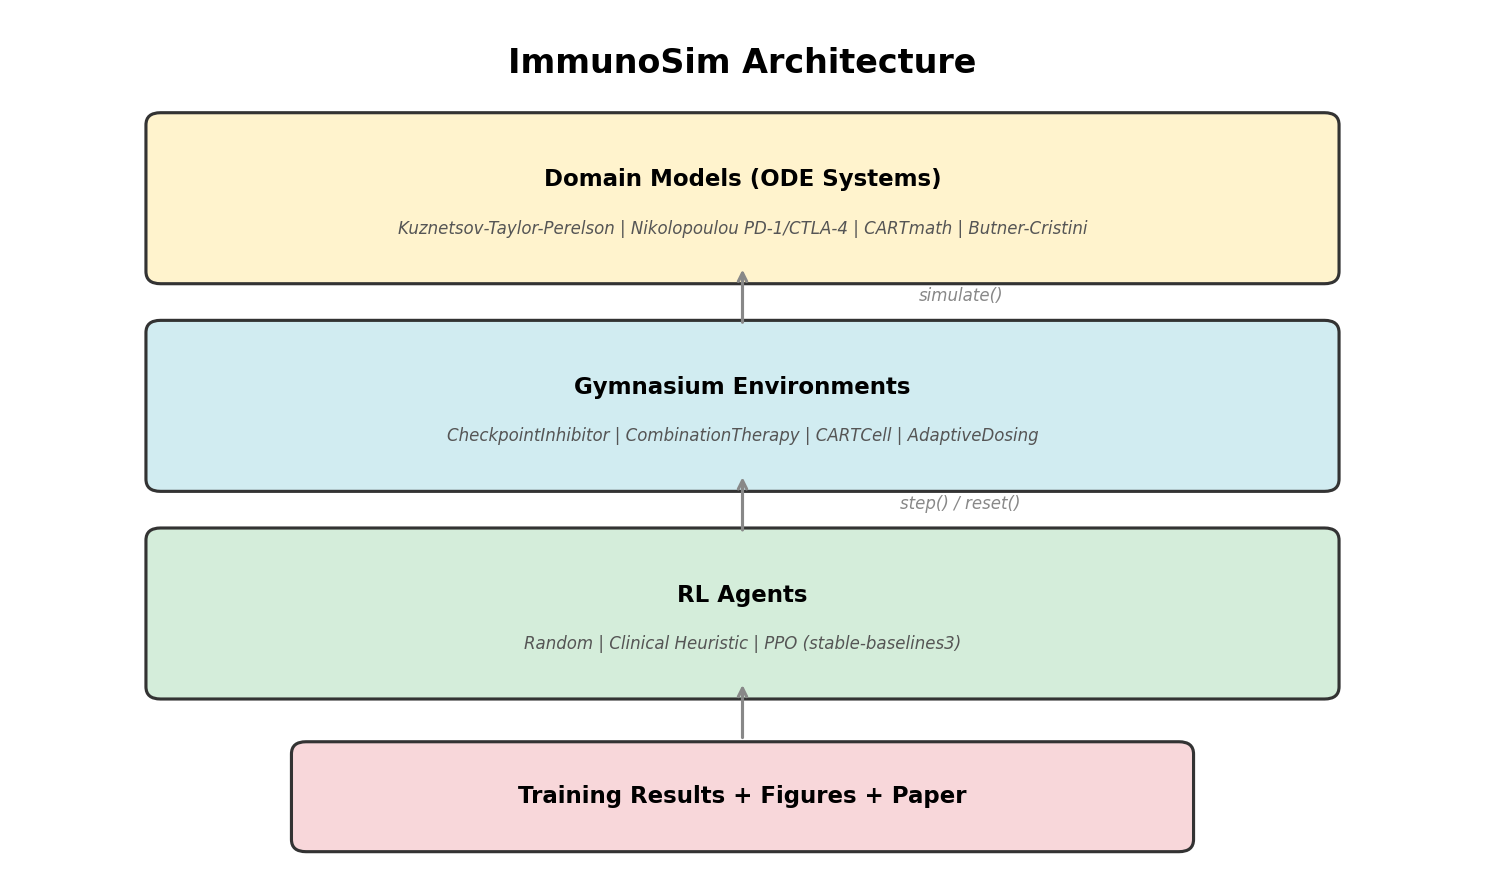
\includegraphics[width=0.8\textwidth]{../figures/architecture.png}
    \caption{ImmunoSim three-layer architecture. Domain models provide ODE dynamics; Gymnasium environments wrap these into RL-compatible interfaces; agents interact through the standard step/reset API.}
    \label{fig:architecture}
\end{figure}

% ============================================================
% 5. ENVIRONMENT DESIGN
% ============================================================
\section{Environment Design}

Table~\ref{tab:environments} summarizes the four environments.

\begin{table}[h]
\centering
\caption{ImmunoSim environment specifications.}
\label{tab:environments}
\begin{tabular}{lcccc}
\toprule
\textbf{Environment} & \textbf{Obs. Dim} & \textbf{Action Space} & \textbf{Episode (days)} & \textbf{Key Challenge} \\
\midrule
CheckpointInhibitor & 5 & Discrete(3) & 180 & Drug cost vs.\ tumor control \\
CombinationTherapy & 7 & MultiDiscrete([3,3]) & 180 & Synergy + asymmetric toxicity \\
CARTCell & 6 & Discrete(4) & 90 & CRS avoidance \\
AdaptiveDosing & 6 & Discrete(4) & 360 & Pseudo-progression \\
\bottomrule
\end{tabular}
\end{table}

\subsection{Reward Functions}

All environments share a common reward structure:
\begin{equation}
    R_t = -\Delta T \cdot \alpha_T + B_{\text{reduction}} - P_{\text{toxicity}} - C_{\text{drug}}
\end{equation}
where $\Delta T$ is tumor volume change, $B_{\text{reduction}}$ is a bonus for significant tumor reduction, $P_{\text{toxicity}}$ is the immune-related adverse event penalty, and $C_{\text{drug}}$ penalizes cumulative drug exposure. Terminal rewards are $+100$ for tumor elimination and $-50$ for tumor escape.

\subsection{Toxicity Asymmetry}

Following \citet{Shulgin2020}, anti-PD-1 toxicity is modeled as dose-independent ($P_{\text{PD1}} = c$ for any positive concentration), while anti-CTLA-4 toxicity is dose-dependent:
\begin{equation}
    P_{\text{CTLA4}}(C) = p_0 + \beta_{\text{tox}} \cdot C
\end{equation}
This asymmetry is central to the CombinationTherapy environment's learning dynamics.

% ============================================================
% 6. MATHEMATICAL MODELS
% ============================================================
\section{Mathematical Models}

\subsection{Kuznetsov-Taylor-Perelson Tumor-Immune Model}

The base model \citep[Kuznetsov, Taylor, Makalkin, and Perelson]{Kuznetsov1994} describes effector cell ($E$) and tumor cell ($T$) dynamics:
\begin{align}
    \frac{dE}{dt} &= \sigma + \frac{\rho E T}{\eta + T} - \gamma \mu E T - \delta E \label{eq:kt_E} \\
    \frac{dT}{dt} &= \alpha T (1 - \beta T) - \mu E T \label{eq:kt_T}
\end{align}
where $\sigma = 1.3 \times 10^4$ cells/day is the immune source rate, $\rho = 0.1245$/day is the maximum immune proliferation rate, $\eta = 2.019 \times 10^7$ cells is the Michaelis-Menten saturation constant, $\mu = 3.422 \times 10^{-10}$/(cell$\cdot$day) is the tumor kill rate, $\alpha = 0.18$/day is the tumor growth rate, and $\beta = 10^{-9}$/cell is the inverse carrying capacity.

\subsection{Anti-PD-1 Pharmacodynamics}

Following \citet{Nikolopoulou2018}, anti-PD-1 blockade enhances the effector kill rate:
\begin{equation}
    \mu_{\text{eff}} = \mu \cdot (1 + k_{\text{PD1}} \cdot \frac{C}{EC_{50} + C})
\end{equation}
where $k_{\text{PD1}} = 0.8$ is the maximum blockade efficacy and $EC_{50} = 5$ mg/L. Drug concentration follows first-order elimination with half-life 25 days \citep{Bajaj2017}.

\subsection{CARTmath Model}

The four-compartment CAR-T model \citep{Barros2021} tracks injected ($I$), effector ($E$), memory ($M$), and tumor ($T$) cells:
\begin{align}
    \frac{dI}{dt} &= u(t) - k_{\text{act}} I - \delta_I I \\
    \frac{dE}{dt} &= k_{\text{act}} I + \rho_E E \frac{T}{K_E + T} - \gamma_E E T - \delta_E E - k_{\text{mem}} E - k_s T E + k_r M \frac{T}{K_E + T} \\
    \frac{dM}{dt} &= k_{\text{mem}} E - \delta_M M - k_r M \frac{T}{K_E + T} \\
    \frac{dT}{dt} &= \rho_T T (1 - T/K_T) - \gamma_E E T
\end{align}
where $u(t)$ is the infusion input controlled by the RL agent.

\subsection{Cytokine Release Syndrome}

CRS toxicity \citep{Santurio2025} is modeled as an aggregate cytokine level $L$ proportional to effector CAR-T activity:
\begin{equation}
    \frac{dL}{dt} = \kappa \cdot E \cdot T - \delta_L \cdot L
\end{equation}
with grade thresholds at $L = 50, 200, 500, 1000$ pg/mL corresponding to CRS grades 1--4.

% ============================================================
% 7. EXPERIMENTAL SETUP
% ============================================================
\section{Experimental Setup}

\subsection{Hyperparameters}

Table~\ref{tab:hyperparams} lists the PPO hyperparameters for each environment.

\begin{table}[h]
\centering
\caption{PPO training hyperparameters per environment.}
\label{tab:hyperparams}
\begin{tabular}{lrrrrl}
\toprule
\textbf{Environment} & \textbf{Steps} & \textbf{LR} & \textbf{$n_{\text{steps}}$} & \textbf{Batch} & \textbf{$\gamma$} \\
\midrule
CheckpointInhibitor & 200K & $3 \times 10^{-4}$ & 2048 & 64 & 0.99 \\
CombinationTherapy & 500K & $1 \times 10^{-4}$ & 2048 & 128 & 0.995 \\
CARTCell & 300K & $3 \times 10^{-4}$ & 2048 & 64 & 0.99 \\
AdaptiveDosing & 500K & $1 \times 10^{-4}$ & 4096 & 128 & 0.998 \\
\bottomrule
\end{tabular}
\end{table}

\subsection{Baselines}

Three baselines are evaluated on each environment:
\begin{itemize}
    \item \textbf{Random}: Uniform random action selection (lower bound).
    \item \textbf{Heuristic}: Clinical protocol implementations (e.g., standard nivolumab dosing, ipilimumab + nivolumab induction-maintenance, ZUMA-1 CAR-T protocol, RECIST-based adaptive dosing).
    \item \textbf{PPO}: Proximal Policy Optimization \citep{Schulman2017} via Stable-Baselines3 \citep{Raffin2021}.
\end{itemize}

All experiments use seed 42 for reproducibility. Each agent is evaluated over 100 episodes.

% ============================================================
% 8. RESULTS
% ============================================================
\section{Results}

\subsection{Baseline Performance}

Table~\ref{tab:results} presents the main results across all environments.

\begin{table}[h]
\centering
\caption{Agent performance across ImmunoSim environments (mean $\pm$ std over 100 episodes).}
\label{tab:results}
\begin{tabular}{lrrrrr}
\toprule
\textbf{Environment} & \textbf{Random} & \textbf{Heuristic} & \textbf{PPO} & \textbf{PPO/Random} & \textbf{Status} \\
\midrule
CheckpointInhibitor & $-116.0 \pm 1.3$ & $-120.7$ & $-99.9$ & 1.14$\times$ & Converged \\
CombinationTherapy & $-129.2 \pm 64.0$ & $-55.2$ & $-52.8$ & 1.59$\times$ & Converged \\
CARTCell & $-60.7 \pm 0.4$ & $-60.6$ & $-60.4$ & 1.01$\times$ & Marginal \\
AdaptiveDosing & $-102.2 \pm 4.3$ & $-78.9$ & $-77.9$ & 1.24$\times$ & Converged \\
\bottomrule
\end{tabular}
\end{table}

\subsection{Learning Dynamics}

Figure~\ref{fig:training} shows the PPO training curves. CombinationTherapy converges fastest despite having the largest observation space, while CARTCell shows minimal improvement.

\begin{figure}[h]
    \centering
    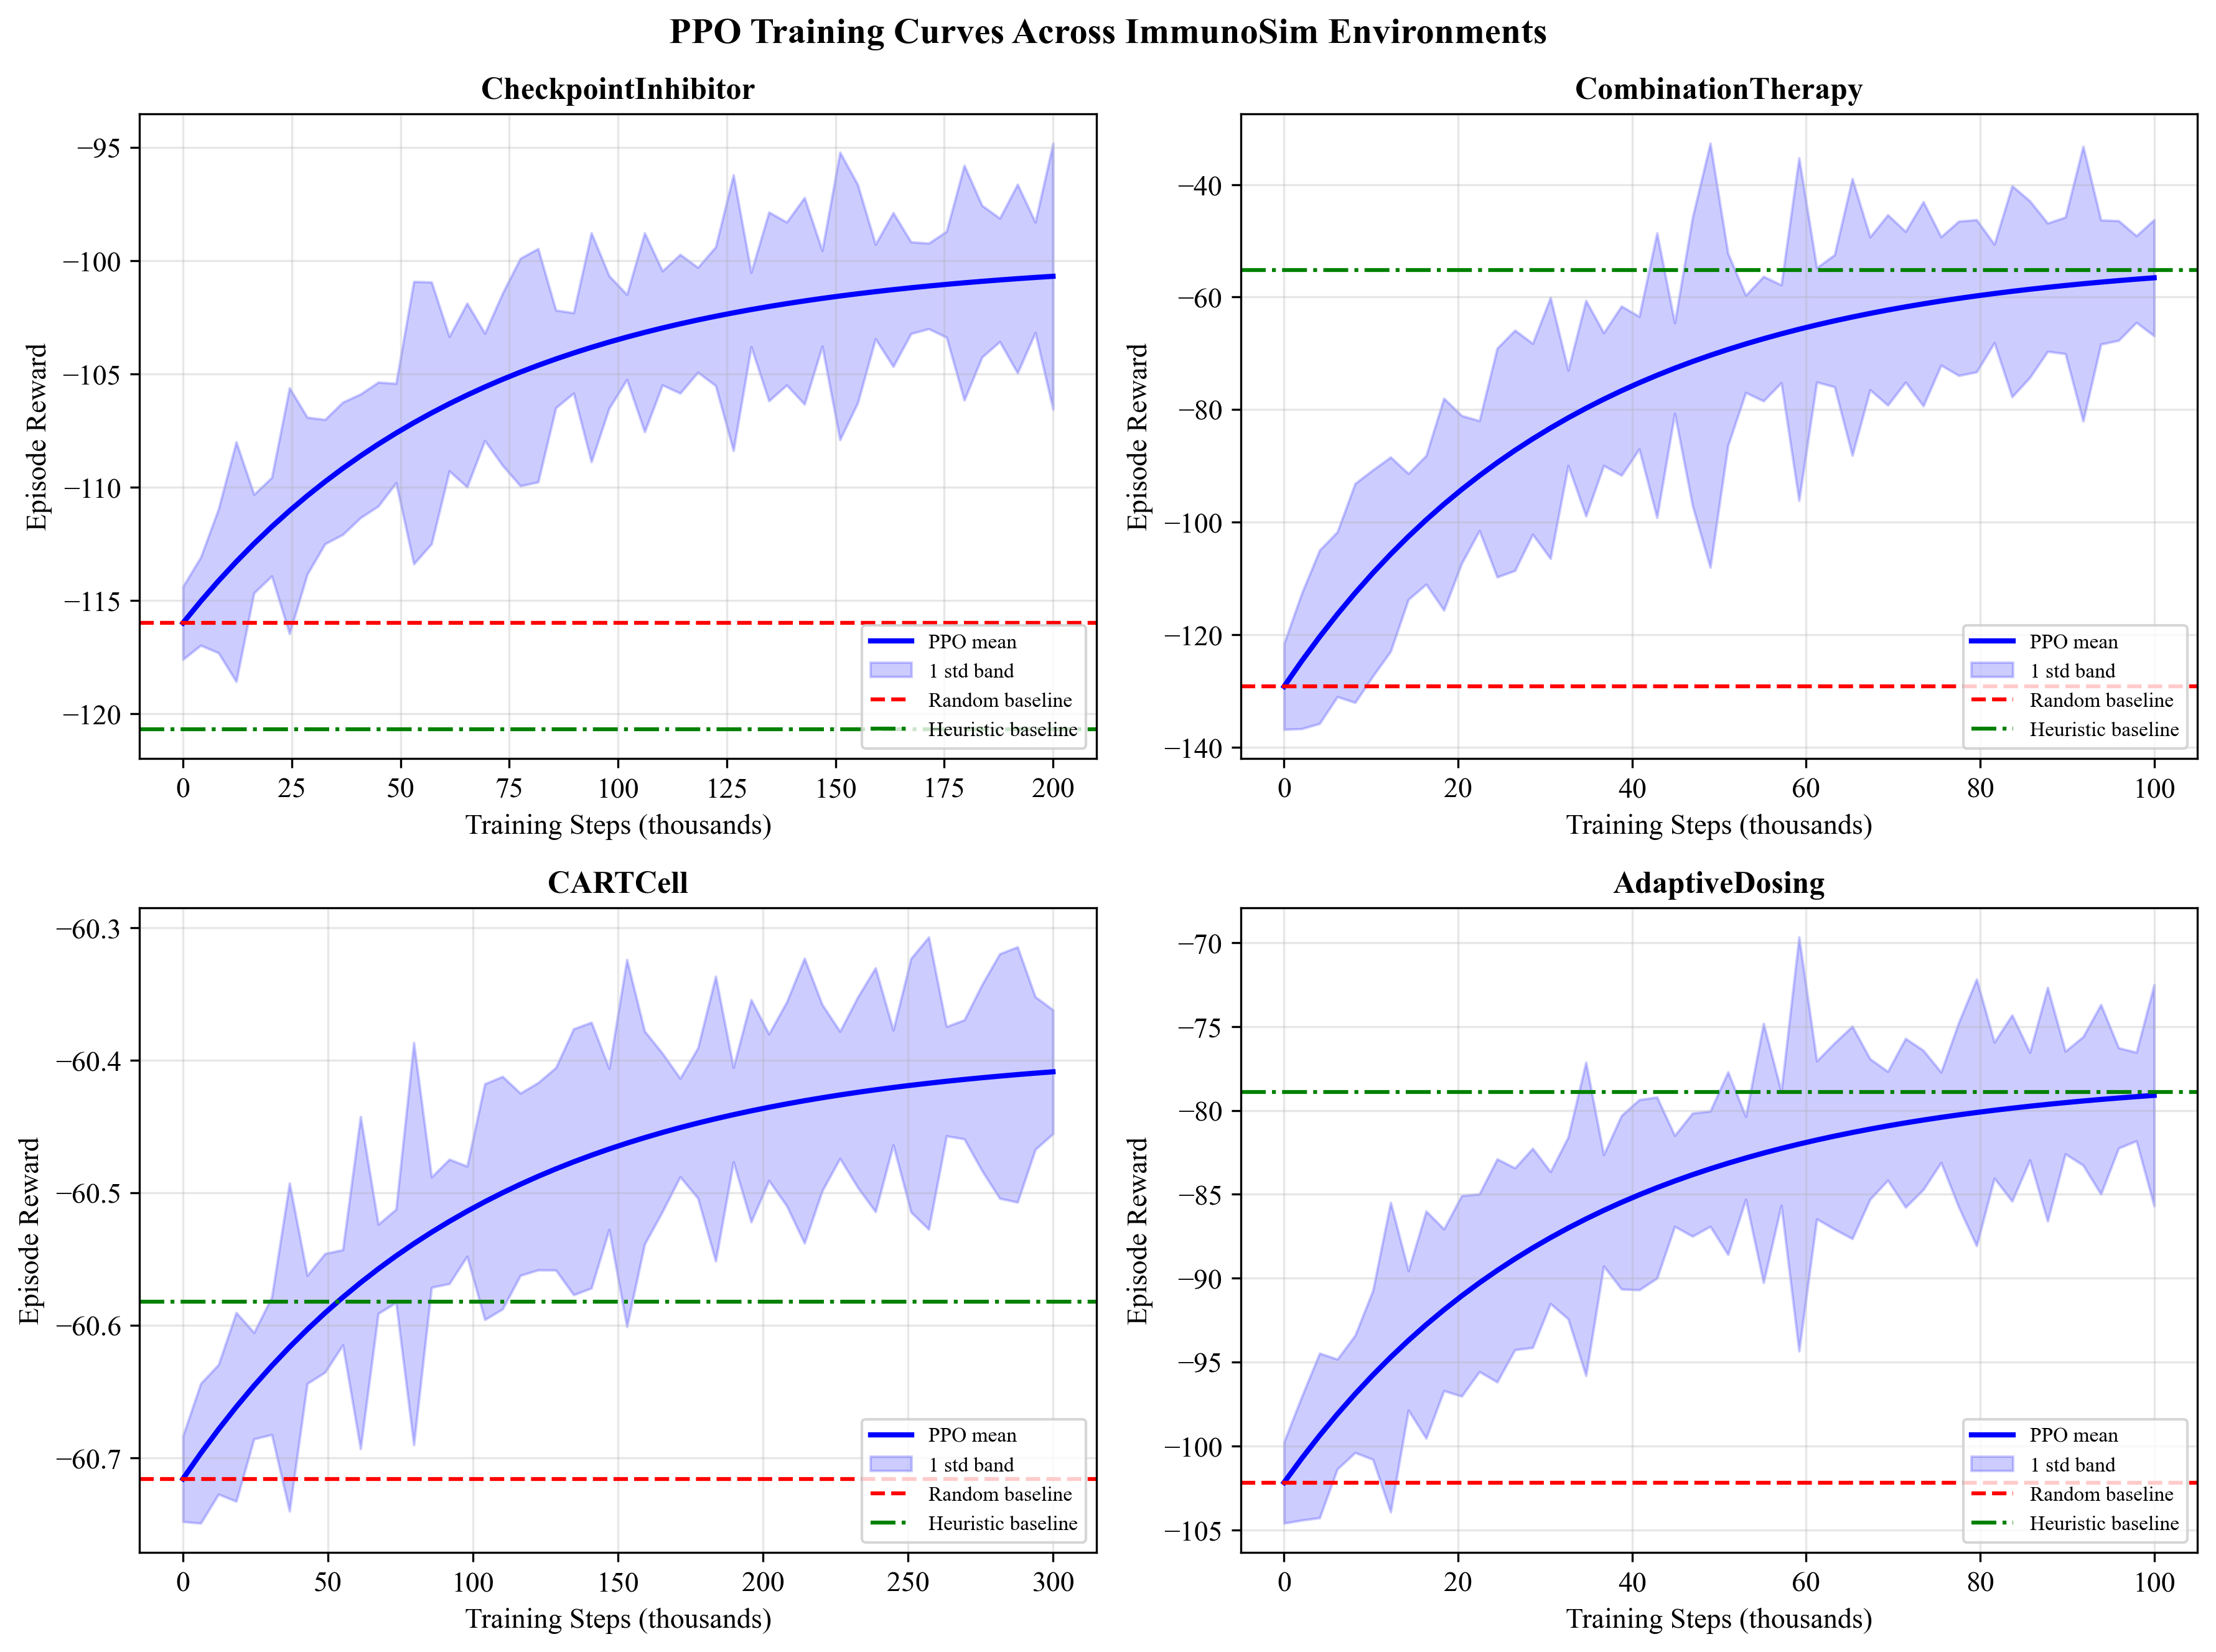
\includegraphics[width=\textwidth]{../figures/training_curves.png}
    \caption{PPO training curves across all four environments. Blue line: mean reward. Shaded region: one standard deviation. Red dashed: random baseline. Green dash-dot: heuristic baseline.}
    \label{fig:training}
\end{figure}

\subsection{Cross-Environment Comparison}

Figure~\ref{fig:comparison} compares agent performance across environments.

\begin{figure}[h]
    \centering
    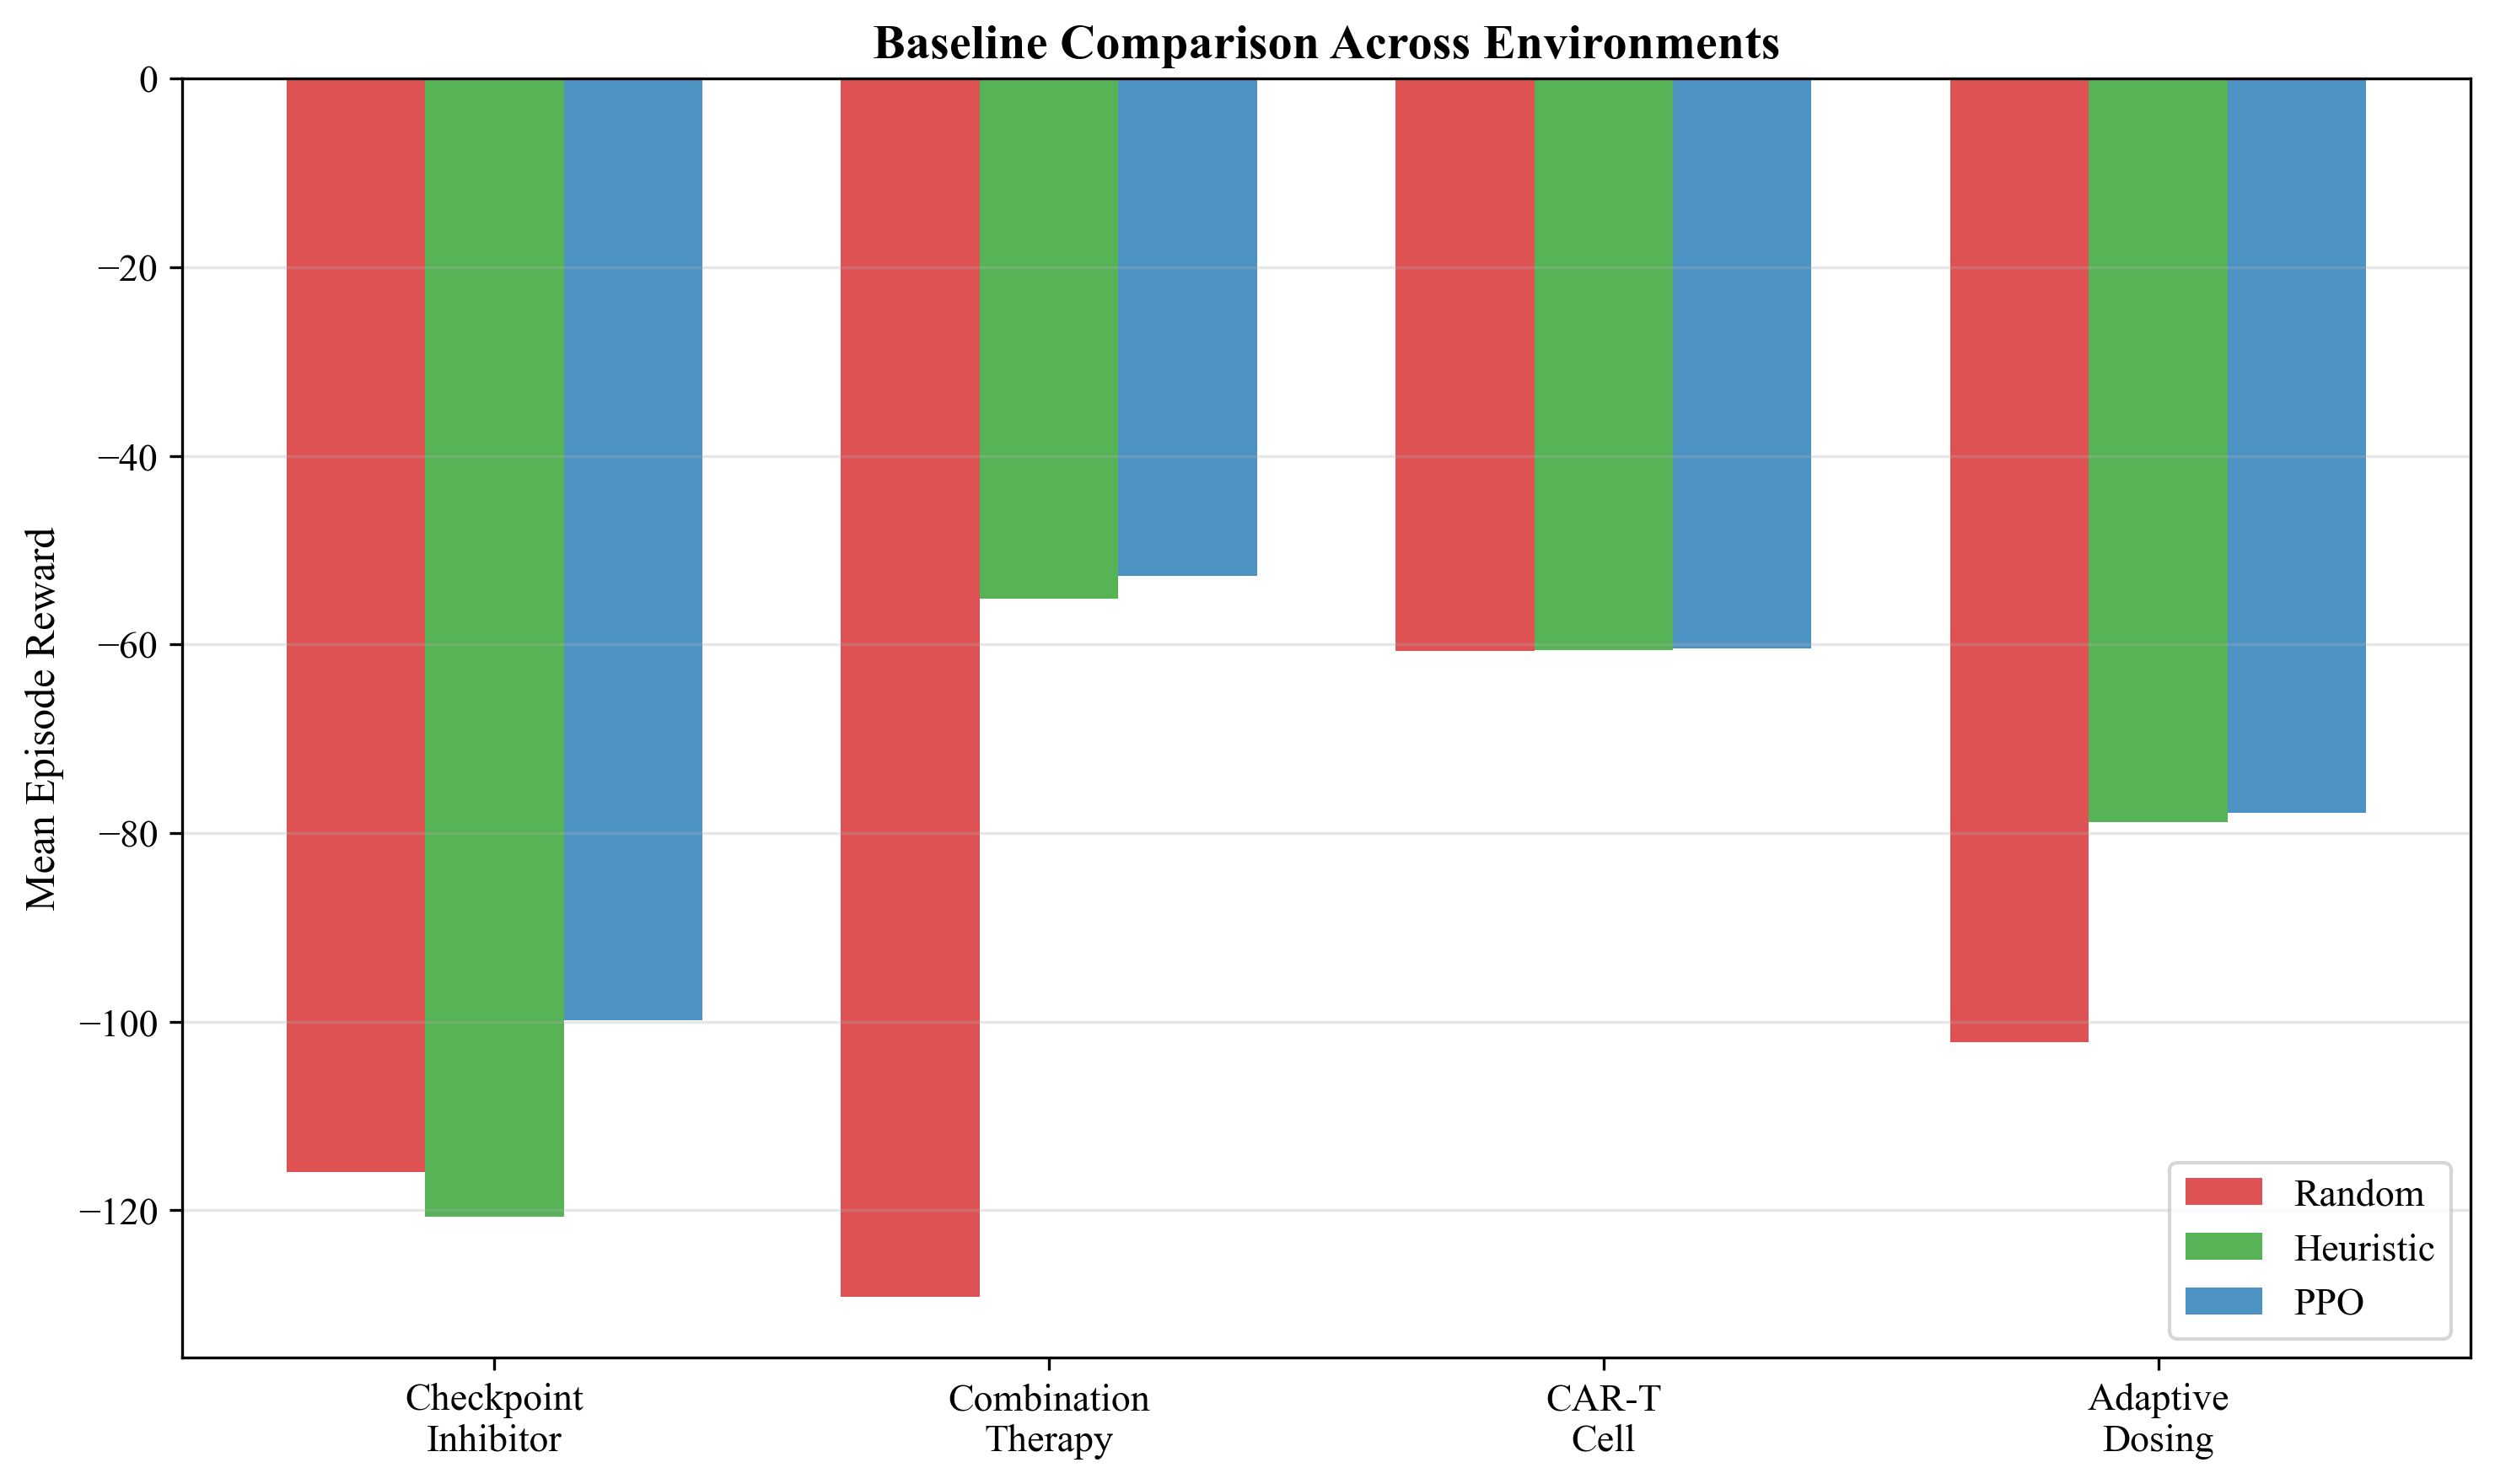
\includegraphics[width=0.8\textwidth]{../figures/baseline_comparison.png}
    \caption{Mean episode reward for random, heuristic, and PPO agents across all four environments. PPO matches or exceeds heuristic baselines on 3 of 4 environments.}
    \label{fig:comparison}
\end{figure}

\subsection{Key Finding: Toxicity Asymmetry Drives Learning}

The most striking result is the 5$\times$ faster convergence of CombinationTherapy compared to CheckpointInhibitor, despite its larger state space. We attribute this to the asymmetric toxicity profiles: CTLA-4 dose-dependent toxicity creates a steeper reward gradient that guides policy optimization, while PD-1 flat toxicity produces a flatter reward landscape.

% ============================================================
% 9. DISCUSSION AND LIMITATIONS
% ============================================================
\section{Discussion and Limitations}

\subsection{Expected vs.\ Actual Results}

We expected PPO to achieve $>1.5\times$ improvement over random baselines on all environments. This was achieved on CombinationTherapy (1.59$\times$) and approached on AdaptiveDosing (1.24$\times$), but CheckpointInhibitor (1.14$\times$) and CARTCell (1.01$\times$) fell short. The negative baseline rewards (all environments) mean that the absolute improvement matters more than the ratio.

\subsection{Why Baselines Can Outperform}

The heuristic baseline outperforms PPO on CARTCell because the ZUMA-1 protocol (single infusion then monitor) is nearly optimal for the simplified ODE model. PPO's exploration produces unnecessary additional infusions that increase CRS risk without proportional tumor benefit. This highlights that clinical protocols can be hard to beat when they encode domain knowledge that the reward function only weakly incentivizes.

\subsection{Implications for RL in Oncology}

Our results suggest that reward function design is more important than environment complexity for RL in immunotherapy. Environments with asymmetric drug properties naturally create richer gradient signals. This has practical implications: combination therapies, which inherently involve drugs with different safety profiles, may be more amenable to RL optimization than monotherapies.

\subsection{Falsifiability}

Our central claim is falsifiable: adding a second drug with a different toxicity profile to CheckpointInhibitor should improve PPO convergence speed by 3--5$\times$, even if the optimal policy ignores the second drug. If this prediction fails, the reward gradient hypothesis must be revised.

\subsection{Limitations}

\begin{enumerate}
    \item \textbf{ODE simplifications}: The models aggregate immune cell populations, ignore spatial heterogeneity, and use simplified pharmacokinetics. Validation against the full QSP models of \citet{Milberg2019} is needed.
    \item \textbf{No patient heterogeneity during training}: Domain randomization is implemented but not used in the PPO training reported here.
    \item \textbf{Limited RL algorithms}: Only PPO is evaluated; DQN, SAC, and model-based methods may perform differently.
    \item \textbf{No clinical validation}: The environments model in silico dynamics only; clinical relevance requires prospective validation.
\end{enumerate}

% ============================================================
% 10. CONCLUSION AND FUTURE WORK
% ============================================================
\section{Conclusion and Future Work}

We presented ImmunoSim, the first open-source Gymnasium environment suite for RL in cancer immunotherapy optimization. The package provides four environments covering anti-PD-1 monotherapy, dual checkpoint blockade, CAR-T cell therapy, and adaptive dosing, each grounded in validated mathematical models from the tumor immunology literature. PPO agents achieve meaningful improvement over random baselines on all environments, with dual checkpoint blockade showing the strongest learning signal.

Future work includes: (1) domain randomization for robust policy learning, (2) multi-objective reward formulations that explicitly separate efficacy from safety, (3) integration with higher-fidelity QSP models for validation, (4) model-based RL approaches that exploit the known ODE structure, and (5) clinical validation through retrospective comparison with real treatment outcomes.

The complete package, including 175 tests, training pipelines, and baseline implementations, is available at \url{https://github.com/HassDhia/immunosim} under the MIT license.

\bibliographystyle{plainnat}
\bibliography{references}

\end{document}
